\documentclass[11pt]{article}
\usepackage[pdftex]{graphicx}
\usepackage{amsmath}

\title{A Survey of Parallelization of Kalman Filters}
\author{
       Brian J Gravelle 
}
\date{\today}


\begin{document}
\maketitle

\begin{abstract}
Kalman Filters have been an important aspect of many computer systems since they were first developed in the 1960s. Many of these applications require real-time speeds which has necessitated the parallelization of the Kalman filter from early in its development. This survey explores efforts to accelerate the algorithm with parallel techniques over the last 30 years  and discusses of the domains to which those parallelizations were applied. Many of the techniques are highly specialized to a particular domain so special care is given to how the parallelizations could be applied to different areas or are restricted to a specific application. Additionally, some discussion of future research is provided.
\end{abstract}

\section{Introduction}
Since their inception in 1960 Kalman filters have been heavily used for the estimation of states in dynamic systems. These filters have numerous applications especially in tracking various objects; they have been used to track objects in conjunction with computer vision, radar tracking for airplanes and ships, vehicle and missile guidance systems, orbit calculation for satellites, and particles in HEP. Additionally, they have been used for demographic and economic studies, industrial process control, climate science, and communication systems. Often these applications, the tracking ones especially, require real-time performance, pushing the performance demands of Kalman filtering.

At first the filtering was done primarily using customized circuits, each designed for the specific application to match the number of states in use. As modern computers developed, new opportunities for flexibility and improved performance were discovered. In many cases parallelism at different levels features in the performance enhancement of the Kalman filter. Commonly the underlying linear algebra calculations are parallelized in one fashion while the broader equations or simultaneous filters are parallelized a different way; however, some of the applications take different approaches as discussed below. In many cases the application area significantly impacts how the filter is parallelized since the number of states varies dramatically between. For this reason we include a discussion of the intended applications alongside the implementations.

In general there are three motivations for parallelizing an Implementation of the Kalman filter. First is for the sake of real-time performance. In many cases, particularly those for tracking, the results must be obtained in real time or else the plane, boat, or subatomic particle will be lost. Second, the number of states involved in the computation is so large that a serial implementation results in unacceptable runtime, as is the case in the climate applications. Lastly the parallelization may be inherent to the system analyzing the data such as sensor networks. In each situation the application has significant impact on the types of parallelism and computational resources available to the programmer. These differences inspire a wide variety of implementations. 

The rest of the paper is not organized but is as follows: Section 2 covers background on the Kalman filter; Section 3 discusses some early implementations of parallel Kalman filters; Section 4 presents more recent implementations and applications; Section 5 talks about Kalman filters parallelized over distributed sensor networks; Section 6 is about FPGA implementations; and Section 7 concludes. I sincerely apologize for the case study of bad writing that this paper is.


\section{Background}
Kalman filters \cite{kalman1960new} were originally presented in 1960 to provide a solution to filtering and prediction problems in dynamic systems. In particular, the results targeted the signal processing involved in communication and control systems. Since then, the Kalman filter has been applied to many dynamic systems in fields including physics, signal processing, economics, and others. In this section, we present some background information to enable the reader to better understand the rest of the survey. Interested readers are directed to the following sources: \cite{blackman1986multiple, welch1995introduction, budhiraja2007survey, kalman1960new}.

The Kalman filter is used to estimate the state of some dynamic system based on measurements, models, and associated errors of that system. This information is combined into a set of matrices that represent the whole system (Table \ref{mats}). The sizes of the matrices are based on the number of states in the system model ($n$) and the number of states measured in each time step ($m$). While some applications have larger state sizes, most require only a small number of states, resulting in matrices that are at the largest 20x20. In addition to the matrices there are also two vectors; $x$ of length $n$ that holds the estimated state and $y$ of length m for the current measurements.

\begin{table}
\caption{List of matrices involved in the Kalman filter.} 
\label{mats}
\centering
\begin{tabular}{||c c c||} 
\hline
Name & Description & dimensions \\ [0.5ex] 
\hline\hline
A & system dynamics & $nxn$\\
\hline
C or H & measurement matrix & $mxn$\\
\hline
Q & process (system) noise & $nxn$\\
\hline
R & measurement noise & $mxm$\\
\hline
P & error covariance & $nxn$\\
\hline
K & Kalman gain & $nxm$\\
\hline
\end{tabular}
\end{table}

At each time step the predicted state and the most recent measurement are compared and these values, combined with the error matrices are used to predict the next state. This prediction is based on weighting the measurement and model (expressed in the Kalman gain) and emphasizing one over the other based on error values. The accuracy of the Kalman filter relies heavily of the accuracy of the error and covariance matrices since these are integral in determining the Kalman gain with each step.

The Kalman equations are shown in Equations 1 - 5. Equations 1 and 2 are the predict portion, estimating the next state based on past data. Equations 3 - 5 and the correct section, updating the estimated state and Kalman gain based on the measurement and predicted state. There are additional versions such as the Extended Kalman Filter and Square Root Kalman Filter that implement improvements such as time variant error functions, or other changes to improve performance or accuracy.

\begin{equation}
\hat{x}_{new} = A\hat{x}
\end{equation}

\begin{equation}
P=APA^T+Q
\end{equation}

\begin{equation}
K = PC^T(CPC^T+R)^{-1}
\end{equation}

\begin{equation}
\hat{x}=\hat{x}_{new} + K(y-C\hat{x}_{new})
\end{equation}

\begin{equation}
P=(I-KC)P
\end{equation}

\section{Early Work}
Since the kalman filter has been around for so long, they have been the subject of many research projects seeking to improve the performance and/or accuracy. Two of the early results are discussed in this section. Both works are intended for Multiple Target Tracking of planes, satellites, or other rapidly moving targets.

\subsection{Circuit Parallelization}
In \cite{Shaffer:1987:IPE:42040.42101}, Shaffer presents a circuit design for an extended Kalman filter. While this work is a hardware implementation rather than software, it still applies the theoretical concepts and parallel patterns that are common in modern parallel software. In particular, Shaffer uses a pipeline pattern to take advantage of the concurrency of the algorithm and streaming nature of the data. Figure \ref{fig:shaffer} shows the data flow diagram of the system.

\begin{figure}
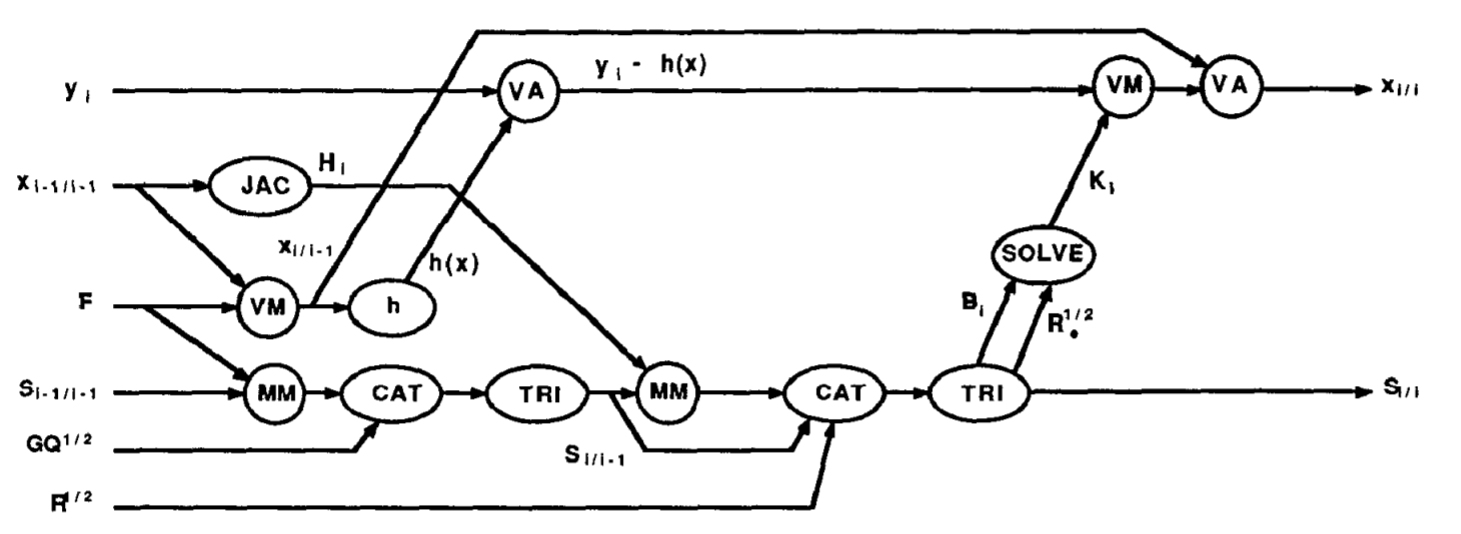
\includegraphics[width=\textwidth]{shaffer.png}
\caption{Dataflow diagram from \cite{Shaffer:1987:IPE:42040.42101}}
\label{fig:shaffer}
\end{figure}

The pipelining of the circuit which was enabled by the removal of recursion from the implementation, resulted in a 360x increase in throughput for the system. This improvement allowed the authors to over 500 targets while collecting 1188 samples/sec.

\subsection{Early Vector Parallelism}
Palis and Krecker, \cite{palis1990parallel}, use the SIMD arrays available in the Connection Machine (a supercomputer manufactured in the late 1980s) to parallelize the work of a single filter and the many-cores of the machine to parallelize the operation of numerous independent filters. The authors use the Square Root Kalman filter which is a variation that allows it to be processed using single-precision calculations without information loss.

The first step to parallelism is to use the SIMD operations to improve the speed of the linear algebra operations. These operations take advantage of the independence of row and elements in matrix operations and can improve the speed of a single Kalman filter operating on a single node. The authors show that the time for computation grows linearly with the number of states in the parallel version rather than cubicly as it does in the serial version. 

Second, the authors demonstrate that when tracking multiple targets the Kalman filters (one or more for each target) can be parallelized by running them on independent processors in the Connection Machine cluster. Their results show that this method can track many more targets than a serial machine.

\section{Modern Implementations and Applications}
Since the early efforts to parallelize the Kalman filter many advances have been made in computer systems that allow further improvements to the performance. Many of these take a similar approach as Palis and Krecker, using SIMD operations for the matrix calculations and threads or processes for each individual filter. A variety of applications and implementations on modern hardware are present in this section.


\subsection{High Energy Physics}
Cerati et al. have published several similar papers \cite{cerati2015kalman,cerati2016kalman,cerati2015traditional} on parallelizing Kalman filters for use at CERN. The physicists utilize Kalman filters to build tracks of subatomic particles during the runs of the LHC. Given the size and speed at which these events occur, the filtering must occur as rapidly as possible. Similar to Shaffer's work in the 90s, these authors explloit two levels of parallelism on XeonPhi; the vector instructions for the matrix operations and the concurrent bulding of multiple tracks.

For parallelization of linear algebra the authors develop their own library that is optimized for small matrix computation of various architectures. They demonstrate that the use of vector instructions or MICs can produce significant speedup in the application.

The task of parallelizing multiple tracks in this scenario is complicated by the fact that the implementation explores all possible tracks in the case the multiple potential matches are found. This results in a pattern more akin to fork join than map. This problem results in challenges for load balancing since it is unknown which tracks will need to branch. The authors handle this challenge by partitioning in terms of physical region so that threads would track all objects within one part of the beam.


\subsection{Climate Science}
In \cite{menard2000assimilation1,menard2000assimilation2,lyster1997parallel}, Lyster, Menard and their collaborators present a parallel implementation of a Kalman filter intended for use analyzing trace chemicals in the atmosphere based on satellite measurements. This data comes in five dimensions and has more than $10^4$ states in the dynamic system. 

The relatively large matrices provide enough enough computation to justify the use of distributed memory computation. In their papers the authors analyze two possible partitioning techniques. The first is to distribute matrix P across the different processors and the latter is to distribute matrix A. Both methods show significant speedup over the serial version. Distribution of the P matrix has slightly better timing achieving a speedup of 434 when comparing 500 processors to the serial implementation. The speedup for a smaller number of processors is shown in figure \ref{fig:climate} but the authors say it scales to at least 500.

\begin{figure}
\centering
\includegraphics[width=0.6\textwidth]{climate.png}
\caption{Speedup from \cite{lyster1997parallel}}
\label{fig:climate}
\end{figure}



\subsection{Smart Grid and GPUs}
Recent developments in smart grid technologies have greatly increased the amount and frequency of data available for power grid management. Kalman filters are an important part of the analysis so Karimipour and Dinavahi present a parallelized system based on the kalman filter in \cite{karimipour2015extended}. For this system the authors utilize a machine with a quad-core processor and GPU. To fully utilize available resources they find three types of parallelism seen in figure \ref{fig:mpdse}: Task parallelism between the different equations, data parallelism from the linear algebra, and Linear solver parallelism (for lack of a better phrase) for the parts that aren't in the Kalman filer.

The authors handle the different types of parallelism much like the others did. Linear algebra is sent to GPUs the exploit the SIMD nature of it, while other computations are kept on the CPU. The power grid operations have an interesting twist since they are running additional linear algebra equations at the same time. Additionally, the power grid systems produce between 171 and 23,151 measurements per time step, so the matrices involved are much larger than those in tracking applications allowing the application to take advantage of the wide vectors available in a GPU.


\begin{figure}
\centering
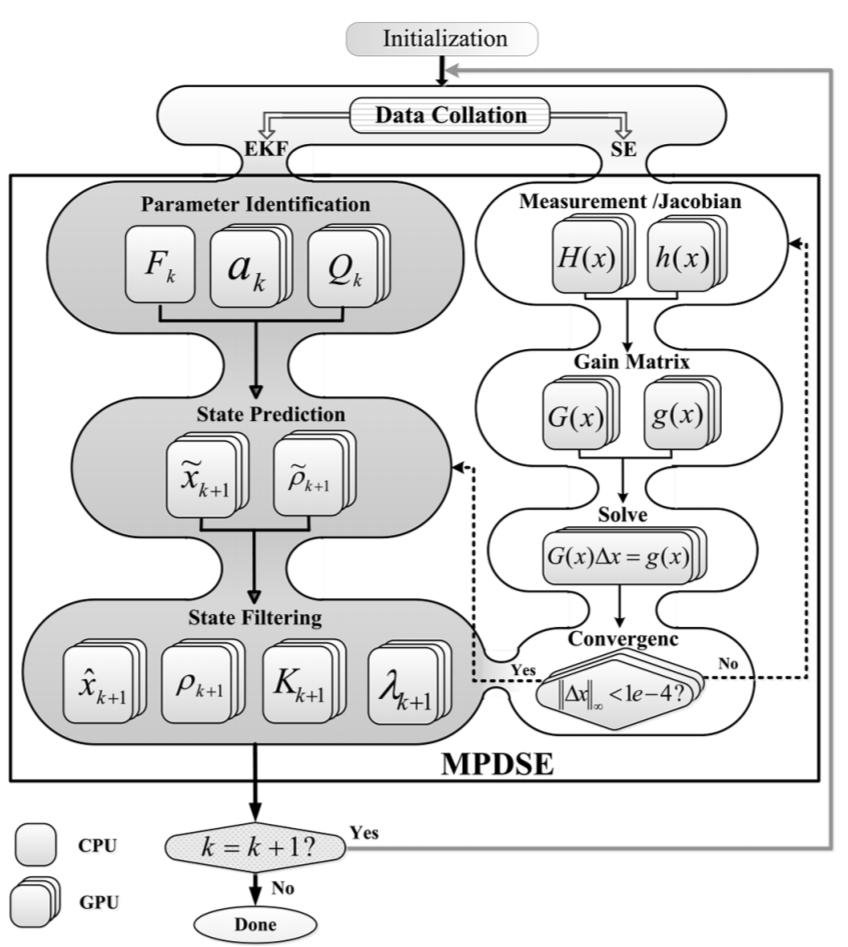
\includegraphics[width=0.6\textwidth]{mpdse.png}
\caption{System flowchart from \cite{karimipour2015extended}}
\label{fig:mpdse}
\end{figure}

\subsection{Cell Phone Management}
Kalman filters play an important role in the processing of MIMO communications such as those used in cell phones. In \cite{rosen2013parallelization}, Rosen et al. present a parallelized implementation of the Kalman filter suitable for modern multicore embedded architectures. The suggested application for this design is for the mapping of cell phone users to cells in the system. This application requires one state per user and all the users over several cells, resulting in hundreds of states.

The authors consider the possibility of separating the equations and running each on a separate core of the processor, but conclude that this idea requires too much communication (particularly of matrix P) to be efficient. Instead, the authors partition the P matrix so that each processor works on all of the equations but only for a section of it. The resulting filter only requires synchronization at the end to bring the results together, so communication among the processors is minimized allowing the authors to maximize communication among cell phones :)

THe authors enable this parallelization by modifying the problem slightly. The full MIMO (multiple input multiple output) problem is broken down into numerous MISO (multiple input single output) problems which limits the number of measurements (possibly to one, the paper wasn't clear) thus eliminating the need to invert a large matrix.

\section{Sensor Applications}
A related but somewhat different application of paralleism in Kalman filters occurs in distributed sensor networks. In these systems each sensor takes some of the measurements but the filter must be computed over all the measurements.  To manage this situation, researchers take different approaches to distributing data and computation. Most use some form of a local computation followed by global, but the details differ between the implementation.

The distributed sensor networks in question fall into two categories with impacts on how the filter is implemented \cite{rao1991fully}. They can have a central node, usually with extra resources available, and a star network where each node connects directly to the central machine. Alternatively the network can be fully distributed, where no central node exists for coordination and the sensors must manage themselves.

\subsection{Central Node}
In the case where the network includes a centralized node, a simple solution would be to have each sensor send its measurement back to the central which could then compute the result as a standard Kalman filter. Distributing all or part of the computation to the nodes can produce improvements in time and resiliency of the computations. 

In \cite{hashemipour1988decentralized}, the authors develop an algorithm for calculating a Kalman filter over such a network. They do this by developing intermediate equations to be executed locally on each node and then compiled into one result at the centralized node. This method allow the system to take advantage of concurrency to improve speed and distribution to be resilient against failure of some nodes. 

Additionally Hashemipour et al consider different sensor configurations . First, they consider collocated sensors where the timing of measurements can be coordinated. In this case the parallelism comes from the fact that measurements impact different parts of the computation so each sensor can have concurrent work. Second they consider the situation where the sensors are widely distributed so measurements are not taken at the same time. In this case, the parallelism exploited comes from the time-sequential feature of the data similar to a pipeline pattern. Lastly the authors demonstrate how to combine the two methods in the situation where several groups of collocated sensor are distributed across a wide area.

\subsection{Fully Distributed}
In \cite{rao1991fully} Rao presents an algorithm for a Kalman filter across a fully distributed group of sensor nodes. In this case there is no centralized node to perform the final computation that brings the local filter results together. To make up for the lack of a central node, the authors simply broadcast the intermediate results to all the node and then every node computes the final result.

Spanos et al present a related system in \cite{spanos2005distributed,spanos2005approximate} that is generalizable to algorithms other than the Klamn filter. Their algorithms allow distributed node to come to a consensus at different points in the algorithm depending on the current network conditions. Their method is similar to Rao's in that it allows the nodes to work independently the n collaborate to get a final result, but achieves even greater resiliency by being flexible in when collaboration occurs. The authors show that the system can compute the filter locally, incorporating data from other sensors as it becomes available with communication occurring $n$ times per filter. 

\section{FPGA Implementations}
While many excellent software applications exist there are also good reasons to implement the Kalman filter using hardware. Two examples,  \cite{bonato2009floating,liu2007efficient}, use FPGA implementations of Kalman filtering to dramatically reduce the time required and the energy used. These implementations employ some level of parallelism but gain further performance benefits by avoiding limitations inherent to software.

Bonato et al. \cite{bonato2009floating}, implement the Extended Kalman filter with the purpose of improving navigation systems for mobile robots.The authors achieve speedup by pipelining the algorithm and ensuring that the most used data (matrix $P$) is the most accessible in the FPGA. Their system has a 3x speedup over a penium processor and consumes 1.3\% of the power. 

Liu et al. \cite{liu2007efficient} apply a similar technique to the Approximate Kalman filter used for feature tracking in computer vision. In this application thousands of features (each with a separate filter) must be tracked at once. The FPGA implementation incorporates enough parallel matrix operation elements that it can perform all or most of the operations simultaneously. Additionally, rather than inverting each matrix the approximate Kalman filter estimates the inversion further minimizing the time.

While FPGA implementations provide fantastic benefits in terms of speed and power they are currently not commonly available to most systems. There has been some talk of incorporating FPGA fabric into standard chips as an adaptable accelerator, so these may become more common in the future. Also for large state-space Kalman filters the size of the hardware may become prohibitive.

\section{Conclusion}
In conclusion, the numerous applications of Kalman filters present varied opportunities for parallelization, but differences in the applications make it challenging to generalize a solution to multiple applications. As a result, there are a variety of creative methods used in parallel Kalman filters. These range from vectorization of the linear algebra to distributing the filter among sensor networks.

Potential future work includes seeking improvements in all of these areas. Notably absent from the research is the use of GPU technology; only the paper on smart grid makes good use of them. The HEP papers mention GPUs repeatedly in future work but have yet to implement anything. GPUs are challenging as the require long vectors or matrices to be effective, but these are unavailable in many of the applications. Vector registers offer a better alternative since they are a more appropriate size, but these to are increasing in length beyond what most tracking applications require. It may be possible to combine the computation for multiple filters into longer vectors that fill the entire vector to achieve the desired speedup. Additional research could be at the higher levels of the application, incorporating the Kalman filters into other parallel structures that offer more concurrency.

\nocite{*}
\bibliographystyle{plain}
\bibliography{filtering}

\end{document}